
%(BEGIN_QUESTION)
% Copyright 2006, Tony R. Kuphaldt, released under the Creative Commons Attribution License (v 1.0)
% This means you may do almost anything with this work of mine, so long as you give me proper credit

The following storage vessel holds a liquid with a density of 57.5 lb/ft$^{3}$.  A pneumatic pressure transmitter located at the bottom infers liquid level by hydrostatic pressure (head).  Determine the calibration range of this pressure transmitter in order to properly translate the range of vessel level (0 to 30 feet) into an output signal of 3 to 15 PSI.  Please express the transmitter's calibration range in units of PSI.

$$\includegraphics[width=15.5cm]{i00244x01.eps}$$

Then, determine the following (assuming the transmitter has been properly calibrated for the application):

\begin{itemize}
\item{} Transmitter output signal (PSI) at 19 feet of level
\item{} Liquid level at 12.4 PSI signal output
\end{itemize}

\underbar{file i00244}
%(END_QUESTION)





%(BEGIN_ANSWER)

Lower range-values (LRV): 0 PSI input = 3 PSI output

\vskip 10pt

Upper range-values (URV): 11.98 PSI input = 15 PSI output

\vskip 10pt

\begin{itemize}
\item{} Transmitter output signal (PSI) at 19 feet of level = 10.6 PSI
\item{} Liquid level at 12.4 PSI signal output = 23.5 feet
\end{itemize}

\vskip 10pt

The 71 $^{o}$F liquid temperature is extraneous information, included for the purpose of challenging students to identify whether or not information is relevant to solving a particular problem.  Liquid temperature is relevant for a level instrument only because changes in temperature can cause the liquid density to change as well, thus influencing the proportionality between liquid height and hydrostatic pressure.  However, since we are already given the density of the liquid in this situation, the temperature is irrelevant.

%(END_ANSWER)





%(BEGIN_NOTES)

%INDEX% Measurement, level: hydrostatic pressure

%(END_NOTES)


